
\centering
\begin{tikzpicture}[node distance=2.5cm]
	
	\proofnode[align=center,font=\small]{root}{$\bot$\\$6$};
	\proofnode[above left of=root,align=center,font=\small]{n3}{$a$\\$3$};
	\proofnode[above right of=root,align=center,font=\small]{n5}{$\neg a$\\$5$};
	\proofnode[above left of=n3,align=center,font=\small]{n1}{$a,\neg b$\\$1$};
	\proofnode[above right of=n3,align=center,font=\small]{n2}{$b$\\$2$};
	\proofnode[above right of=n5,align=center,font=\small]{n4}{$\neg a, \neg b$\\$4$};
	\drawchildren{n5}{n2}{n4};
	\drawchildren{root}{n3}{n5};
	\drawchildren{n3}{n1}{n2};
	
\end{tikzpicture}

